% Drawing 147/09-2 -- folder 147, batch 09, archive page 180 (PDF page 181).
% Transcription: un disque hachuré, deux points marqués sur son bord.
% Kind: hatched disc with boundary points. Method 2 (schematic redraw from the facsimile). Status: ok.
% Notes: A hatched disc with two marked points on its boundary (left, and lower right).
% Coordinates: 1 unit = 1 mm = 1/100 of the crop width (bbox in page fractions: [0.54, 0.686, 0.644, 0.759]).
% Redrawn by Claude (claude-opus-5-5), issue #73, 2026-11-07; not checked by a human; not compiled (no TeX in the session).
% Rights: reproduces part of the work -- behind RENDER_TRANSCRIPTS, never published by itself.
\documentclass[tikz,border=3pt]{standalone}
\usepackage{amsmath,amssymb}
\usetikzlibrary{patterns,arrows.meta}
\tikzset{pencil/.style={black!45}, struck/.style={black!35}, mark/.style={circle,draw,inner sep=1.3pt}, pt/.style={circle,fill,inner sep=0.9pt}, opt/.style={circle,draw,fill=white,inner sep=1.1pt}}
\begin{document}
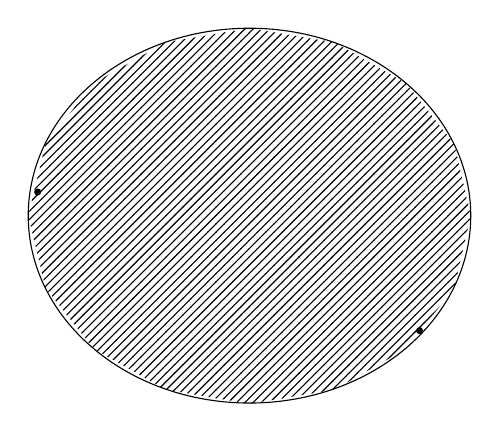
\begin{tikzpicture}[x=1mm,y=1mm,line cap=round,line join=round,font=\scriptsize]
\draw (54.6,-63.8) ellipse[x radius=28.1, y radius=23.8];
\fill[pattern=north east lines] (82.7,-63.8) -- (80.6,-73) -- (74.5,-80.7) -- (65.4,-85.9) -- (54.6,-87.7) -- (43.9,-85.9) -- (34.8,-80.7) -- (28.7,-73) -- (26.5,-63.8) -- (28.7,-54.7) -- (34.8,-47) -- (43.9,-41.8) -- (54.6,-40) -- (65.4,-41.8) -- (74.5,-47) -- (80.6,-54.7) -- cycle;
\node[pt] at (27.7,-60.8) {};
\node[pt] at (76.2,-78.4) {};
\end{tikzpicture}
\end{document}
